%!TEX root = ../../report.tex
\chapter{Leaning Curves}
\label{appendix:learning_curves}
The estimated $\lambda$ values are shown in figure \ref{fig:all_learnings_sim_1} and \ref{fig:all_learnings_sim_2}. The estimated values in the plots are calculated by the average estimate in an area around the obstacles. The requirement for a cell to be used in the average was all parameters, the state and event scores, were above 0.5. As this method deviates from the scoring method used for comparison the result are not directly comparable.
The figures gives an overview of the speed of leaning but as many cells are included that might mainly learn based on noise is may not represent an accurate image of the learning accuracy.


\begin{figure}[htbp]
	\begin{subfigure}[t]{0.5\linewidth}
		\centering
		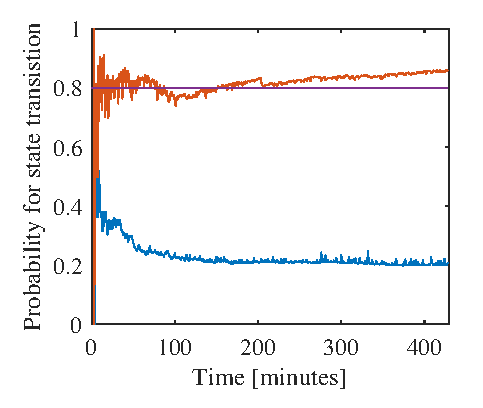
\includegraphics[width=1\linewidth]{chapters/appendix/figures/learning_curves/obs1}
		\caption{Obstacle number 1}
	\end{subfigure}
	\hspace*{\fill}
	\begin{subfigure}[t]{0.5\linewidth}
		\centering
		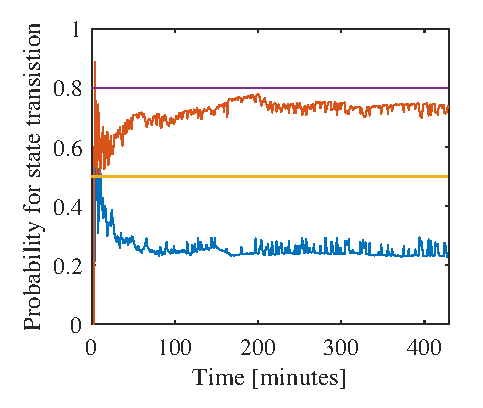
\includegraphics[width=1\linewidth]{chapters/appendix/figures/learning_curves/obs2}
		\caption{Obstacle number 2}
	\end{subfigure}


	\begin{subfigure}[t]{0.5\linewidth}
		\centering
		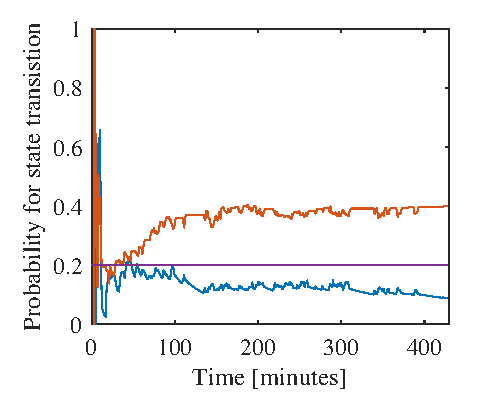
\includegraphics[width=1\linewidth]{chapters/appendix/figures/learning_curves/obs3}
		\caption{Obstacle number 3}
	\end{subfigure}
	\hspace*{\fill}
	\begin{subfigure}[t]{0.5\linewidth}
		\centering
		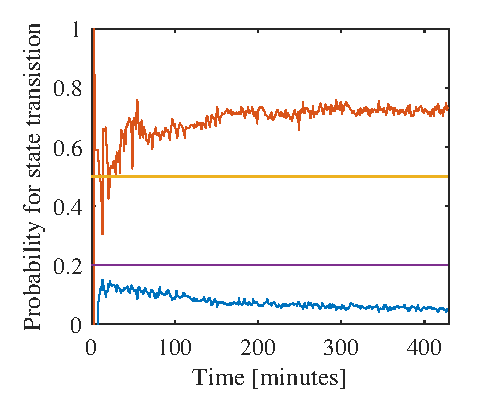
\includegraphics[width=1\linewidth]{chapters/appendix/figures/learning_curves/obs4}
		\caption{Obstacle number 4}
	\end{subfigure}
	
	\hspace*{\fill}
	\begin{subfigure}[t]{0.5\linewidth}
		\centering
		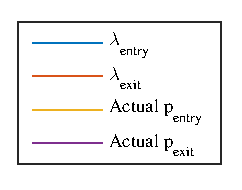
\includegraphics[scale = 1]{chapters/appendix/figures/learning_curves/legend}
		
	\end{subfigure}
	\hspace*{\fill}

	\caption{CAPTION}
	\label{fig:all_learnings_sim_1}
\end{figure}

\begin{figure}[htbp]
	\begin{subfigure}[t]{0.5\linewidth}
		\centering
		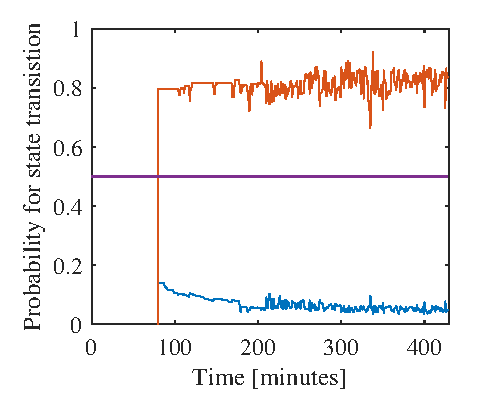
\includegraphics[width=1\linewidth]{chapters/appendix/figures/learning_curves/obs5}
		\caption{Obstacle number 5}
	\end{subfigure}
	\hspace*{\fill}
	\begin{subfigure}[t]{0.5\linewidth}
		\centering
		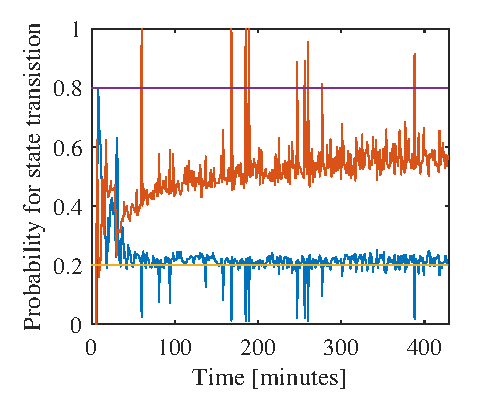
\includegraphics[width=1\linewidth]{chapters/appendix/figures/learning_curves/obs6}
		\caption{Obstacle number 6}
	\end{subfigure}
	
	\begin{subfigure}[t]{0.5\linewidth}
		\centering
		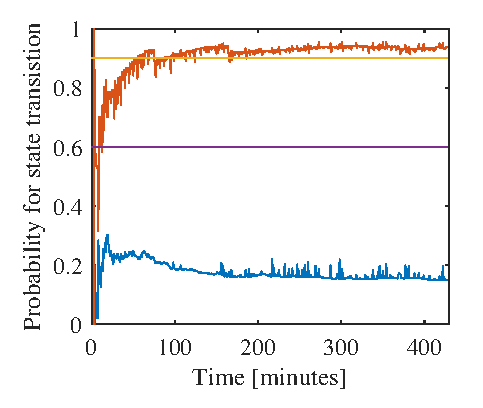
\includegraphics[width=1\linewidth]{chapters/appendix/figures/learning_curves/obs7}
		\caption{Obstacle number 7}
	\end{subfigure}
	\hspace*{\fill}
	\begin{subfigure}[t]{0.5\linewidth}
		\centering
		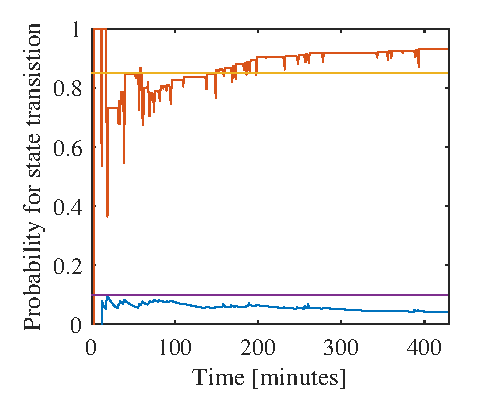
\includegraphics[width=1\linewidth]{chapters/appendix/figures/learning_curves/obs8}
		\caption{Obstacle number 8}
	\end{subfigure}


	\begin{subfigure}[t]{0.5\linewidth}
		\centering
		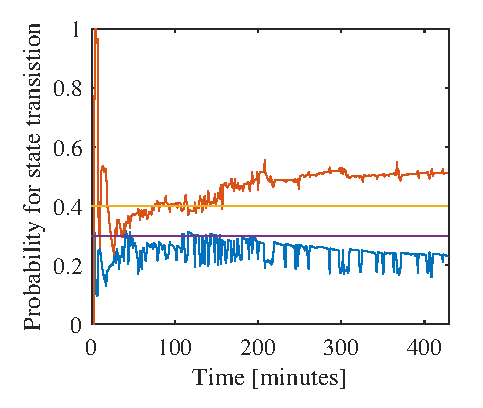
\includegraphics[width=1\linewidth]{chapters/appendix/figures/learning_curves/obs9}
		\caption{Obstacle number 9}
	\end{subfigure}
	\hspace*{\fill}
	\begin{subfigure}[t]{0.5\linewidth}
		\centering
		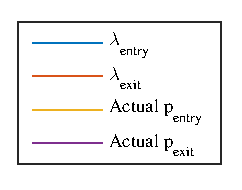
\includegraphics[scale = 1]{chapters/appendix/figures/learning_curves/legend}
	\end{subfigure}

	\caption{CAPTION}
	\label{fig:all_learnings_sim_2}
\end{figure}

\chapter{PMAC Pseudo Code}
\label{appendix:pmac_pseudo_code}
\begin{algorithm}
	\caption{PMAC learning for occupied observations}
	\label{al:object_recognition}
	\begin{algorithmic}[1]
		\State $\mu$ = \{sum, count\}
		\ForAll{observations}
		\If {Observation = occupied}
		\State $s_{score}^{occupied} = s_{score}^{occupied}$ + $s_{score}^{observation}$
		\If {previous state = free}
		\State Clear $\mu_{exit}^{last}$
		\If $\mu_{entry}^{new} > \mu_{entry}^{old}$ 
		\State Clear $\mu_{entry}^{old}$
		\State $e_{entry}^{max} = \mu_{entry}^{new}$
		\Else
		\State $e_{entry}^{max} = \mu_{entry}^{new}$
		\EndIf
		\EndIf
		\State Add observation to $\mu_{exit}^{new}$ and $\mu_{exit}^{old}$
		\If $e_{entry}^{max} > 0$
		\State $e_{score}^{entry} = e_{score}^{entry} + min(s_{score}^{observation},e_{entry}^{max})$
		\State $e_{entry}^{max} = e_{entry}^{max} - min(s_{score}^{observation},e_{entry}^{max})$
		\State $\mu_{entry}^{old}(sum) = \mu_{entry}^{old}(sum) - min(s_{score}^{observation},e_{entry}^{max})$
		\EndIf
		\EndIf
		\If {Observation = free}
			\State Handled similarly to above, but $occupied \leftrightarrow free$ and $entry \leftrightarrow exit$ are switched
		\EndIf
		\EndFor
	\end{algorithmic}
\end{algorithm}


\chapter{USB content}
\label{appendix:usb_content}
The USB flash drive accompanying the printed thesis contains:

\begin{itemize}
	\item Code 
	\begin{itemize}
		\item activity\_layer - The activity layer of the Dynamic mapping system
		\item layered\_costmap\_2d - Modified layered costmap 2d
		\item occupancy\_image\_publisher - Node for publishing occupancy grid as heatmap color images
		\item user\_priority\_map - The user priority layer of the Dynamic mapping system
	\end{itemize}
	\item Logged tests (ROS Bags)
	\begin{itemize}
		\item Learning Markov parameter test data
		\item Localization accuracy
		\item Static mapping simulation
		\item Scan AS
	\end{itemize}
	\item Simulations
	\item The thesis in PDF format
\end{itemize}

The code provided 